%% Creator: Inkscape inkscape 0.48.4, www.inkscape.org
%% PDF/EPS/PS + LaTeX output extension by Johan Engelen, 2010
%% Accompanies image file 'grasp_success_circular.pdf' (pdf, eps, ps)
%%
%% To include the image in your LaTeX document, write
%%   \input{<filename>.pdf_tex}
%%  instead of
%%   \includegraphics{<filename>.pdf}
%% To scale the image, write
%%   \def\svgwidth{<desired width>}
%%   \input{<filename>.pdf_tex}
%%  instead of
%%   \includegraphics[width=<desired width>]{<filename>.pdf}
%%
%% Images with a different path to the parent latex file can
%% be accessed with the `import' package (which may need to be
%% installed) using
%%   \usepackage{import}
%% in the preamble, and then including the image with
%%   \import{<path to file>}{<filename>.pdf_tex}
%% Alternatively, one can specify
%%   \graphicspath{{<path to file>/}}
%% 
%% For more information, please see info/svg-inkscape on CTAN:
%%   http://tug.ctan.org/tex-archive/info/svg-inkscape
%%
\begingroup%
  \makeatletter%
  \providecommand\color[2][]{%
    \errmessage{(Inkscape) Color is used for the text in Inkscape, but the package 'color.sty' is not loaded}%
    \renewcommand\color[2][]{}%
  }%
  \providecommand\transparent[1]{%
    \errmessage{(Inkscape) Transparency is used (non-zero) for the text in Inkscape, but the package 'transparent.sty' is not loaded}%
    \renewcommand\transparent[1]{}%
  }%
  \providecommand\rotatebox[2]{#2}%
  \ifx\svgwidth\undefined%
    \setlength{\unitlength}{201.33696562bp}%
    \ifx\svgscale\undefined%
      \relax%
    \else%
      \setlength{\unitlength}{\unitlength * \real{\svgscale}}%
    \fi%
  \else%
    \setlength{\unitlength}{\svgwidth}%
  \fi%
  \global\let\svgwidth\undefined%
  \global\let\svgscale\undefined%
  \makeatother%
  \begin{picture}(1,0.49955409)%
    \put(0,0){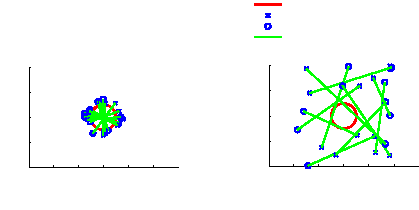
\includegraphics[width=\unitlength]{grasp_success_circular.pdf}}%
    \put(0.67432804,0.07989704){\makebox(0,0)[lb]{\smash{-0.2}}}%
    \put(0.73425495,0.07989704){\makebox(0,0)[lb]{\smash{-0.1}}}%
    \put(0.81421346,0.07989704){\makebox(0,0)[lb]{\smash{0}}}%
    \put(0.86579378,0.07989704){\makebox(0,0)[lb]{\smash{0.1}}}%
    \put(0.92555283,0.07989704){\makebox(0,0)[lb]{\smash{0.2}}}%
    \put(0.59720796,0.0967569){\makebox(0,0)[lb]{\smash{-0.2}}}%
    \put(0.59720796,0.15668301){\makebox(0,0)[lb]{\smash{-0.1}}}%
    \put(0.62558574,0.21660992){\makebox(0,0)[lb]{\smash{0}}}%
    \put(0.60889335,0.27653724){\makebox(0,0)[lb]{\smash{0.1}}}%
    \put(0.60889335,0.33646255){\makebox(0,0)[lb]{\smash{0.2}}}%
    \put(0.8157158,0.05602627){\makebox(0,0)[lb]{\smash{x}}}%
    \put(0.58352024,0.2187797){\rotatebox{90}{\makebox(0,0)[lb]{\smash{y}}}}%
    \put(0.10130414,0.07702147){\makebox(0,0)[lb]{\smash{-0.2}}}%
    \put(0.16123106,0.07702147){\makebox(0,0)[lb]{\smash{-0.1}}}%
    \put(0.24118956,0.07702147){\makebox(0,0)[lb]{\smash{0}}}%
    \put(0.29276988,0.07702147){\makebox(0,0)[lb]{\smash{0.1}}}%
    \put(0.35252893,0.07702147){\makebox(0,0)[lb]{\smash{0.2}}}%
    \put(0.02418406,0.09388132){\makebox(0,0)[lb]{\smash{-0.2}}}%
    \put(0.02418406,0.15380743){\makebox(0,0)[lb]{\smash{-0.1}}}%
    \put(0.05256185,0.21373434){\makebox(0,0)[lb]{\smash{0}}}%
    \put(0.03586945,0.27366166){\makebox(0,0)[lb]{\smash{0.1}}}%
    \put(0.03586945,0.33358697){\makebox(0,0)[lb]{\smash{0.2}}}%
    \put(0.2426919,0.0531507){\makebox(0,0)[lb]{\smash{x}}}%
    \put(0.01049634,0.21590412){\rotatebox{90}{\makebox(0,0)[lb]{\smash{y}}}}%
    \put(0.68353063,0.48415812){\makebox(0,0)[lb]{\smash{object}}}%
    \put(0.6842683,0.45611067){\color[rgb]{0,0,0}\makebox(0,0)[lb]{\smash{left finger tip}}}%
    \put(0.6838491,0.43333901){\color[rgb]{0,0,0}\makebox(0,0)[lb]{\smash{right finger tip}}}%
    \put(0.6827665,0.40853162){\color[rgb]{0,0,0}\makebox(0,0)[lb]{\smash{gripper close direction}}}%
    \put(0.20716763,0.00523842){\color[rgb]{0,0,0}\makebox(0,0)[lb]{\smash{(a)}}}%
    \put(0.78343449,0.0109469){\color[rgb]{0,0,0}\makebox(0,0)[lb]{\smash{(b)}}}%
  \end{picture}%
\endgroup%
